
%\title{EMC LaTeX Portrait Poster Template}
%%%%%%%%%%%%%%%%%%%%%%%%%%%%%%%%%%%%%%%%%
% a1poster Portrait Poster
% LaTeX Template
% Version 2.0 (22/06/16)
%
% The a1poster class was created by:
% Joe Rowing (JoeRowing@exeterms.ac.uk)
% 
% This template has been produced by:
% Joe Rowing at Exeter Mathematics School
%
% License:
% CC BY-NC-SA 3.0 (http://creativecommons.org/licenses/by-nc-sa/3.0/)
%
%%%%%%%%%%%%%%%%%%%%%%%%%%%%%%%%%%%%%%%%%

%----------------------------------------------------------------------------------------
%   PACKAGES AND OTHER DOCUMENT CONFIGURATIONS
%----------------------------------------------------------------------------------------

\documentclass[a0,portrait]{a0poster}

\usepackage{multicol} % This is so we can have multiple columns of text side-by-side
\columnsep=50pt % This is the amount of white space between the columns in the poster
\columnseprule=0.01pt % This is the thickness of the black line between the columns in the poster

\usepackage[svgnames]{xcolor} % Specify colors by their 'svgnames', for a full list of all colors available see here: http://www.latextemplates.com/svgnames-colors

\usepackage{times} % Use the times font
\usepackage{amsmath,amsthm,amssymb,latexsym} % For including math equations, theorems, symbols, etc
\usepackage{mathtools}
\usepackage{hyperref}
\usepackage{cleveref}
\usepackage{autonum}
\usepackage{braket}
\usepackage{cancel}

\usepackage{graphicx} % Required for including images
\graphicspath{{figures/}} % Location of the graphics files
\usepackage{booktabs} % Top and bottom rules for table
\usepackage[font=small,labelfont=bf]{caption} % Required for specifying captions to tables and figures
\usepackage{amsfonts, amsmath, amsthm, amssymb} % For math fonts, symbols and environments
\usepackage{wrapfig} % Allows wrapping text around tables and figures

\begin{document}

%----------------------------------------------------------------------------------------
%   POSTER HEADER 
% The header is divided into two boxes:
% The first is 75% wide and houses the title, subtitle, names, university/organization and contact information
% The second is 25% wide and houses the EMS Logo
% 
%----------------------------------------------------------------------------------------
\begin{minipage}[b]{0.15\linewidth}

\includegraphics[height=10cm]{unmsm.pdf}\\
\end{minipage}
\begin{minipage}[b]{0.7\linewidth}

\begin{center}
\huge\textit{XXVIII Simposio Peruano de F\'isica}\\[1cm] % Subtitle
\Huge \color{DarkRed} \textbf{Probability of False Vacuum Decay in a Scalar Field} \color{Black}\\ % Title  % Title
%\huge\textit{With a subtitle here}\\[1cm] % Subtitle
\large \textbf{$^1$Erwin Renzo Franco Diaz \& Teófilo Vargas Aucalla}\\[0.5cm] % Author(s)
\large Facultad de Ciencias Fı́sicas, Universidad Nacional Mayor de San Marcos, Calle Germ\'an Am\'ezaga 375, Lima, Per\'u\\[0.2cm] % University/organization
\texttt{$^1$erwin.franco1@unmsm.edu.pe}\\
\end{center}

\end{minipage}
%
\begin{minipage}[b]{0.15\linewidth}

\includegraphics[height=10cm]{gft.pdf}\\
\end{minipage}


\vspace{.5cm} % A bit of extra whitespace between the header and poster content

%----------------------------------------------------------------------------------------

\begin{multicols}{3} 
\section{Introduction}
\begin{wrapfigure}{r}{0.15\textwidth}
	%this figure will be at the right
	\caption{Potential with a false minima}
	\label{potencial} 
	\centering
	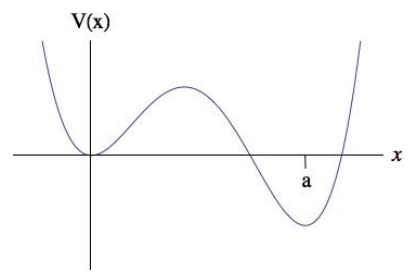
\includegraphics[width=0.15\textwidth]{potencial.png}
\end{wrapfigure}
Classically, a field (or a particle) in a potential with two distinct minima, like the one in \ref{potencial}, is stable in any of them. On the other hand, in a quantum field theory, the minima at $0$ is unstable due to quantum fluctuations and would decay to the state with energy corresponding to the absolute minimum through quantum tunneling, making the other a false vacuum . 


The probability of tunneling through the potential barrier can be obtained by using the semiclassical approximation and has an exponential form \cite{coleman}
\begin{equation}\label{decay}
\Gamma = A e^{-B/\hbar} (1 + O(\hbar))
\end{equation}

Using the Euclidean time formalism and the saddle point approximation for path integrals, $A$ and $B$ are calculated, first in quantum mechanics and then, by analogy, for the scalar field. 

\section{Barrier Penetration in Quantum Mechanics}
In one dimensional quantum mechanics, the coefficient $B$ in \eqref{decay} is given by
\begin{equation}\label{B}
B = 2 \int_{0}^{q_0} \sqrt{2V(q)}dq.
\end{equation}
For convenience, the false minima of the potential is located at 0 where $V(0) = 0$ and $q_0$ is point near the absolute minimum where $V(0) = 0$ again. 

Going into imaginary time $t \rightarrow -i\tau$ (also known as a Wick rotation), the Euclidean time action $S_E$ is obtained
\begin{equation}\label{eucliaction}
S_E =  \int \left[ \frac{1}{2}\left(\frac{dq}{d\tau}\right)^2 + V(q) \right] dt
\end{equation}
The corresponding equation of motion is
\begin{equation}
\frac{d^2 q}{d\tau^2} = \frac{dV}{dq} = -\frac{d(-V)}{dq}
\end{equation}
which can be interpreted as a particle moving in real time in a potential $-V(q)$, and the Euclidean energy of the particle is
\begin{equation}
\mathcal{E} =  \frac{1}{2}\left(\frac{dq}{d\tau}\right)^2 - V(q)
\end{equation}

The solution with an Euclidean action that corresponds to \eqref{B} is the one where the particle that starts in the origin at $\tau = -\infty$, gets to $q_0$ and returns to the origin at $\tau = +\infty$, with $\mathcal{E} = 0$. Because it comes and goes, it is called the "bounce" solution $q_B$. Due to the time translation invariance we can choose any moment in time as the one when the particle reaches $q_0$. For convenience it is chosen to be $\tau = 0$. The velocity of the particle is zero at this time. 

Using the condition $\mathcal{E} = 0$ in \eqref{eucliaction}, taking into account that the motion of the particle for positive $\tau$ is the time reversal of the one for negative $\tau$, and making a change of variable from $\tau$ to $q_B$, the Euclidean action for the bounce $S_B$ can be written as

\begin{equation}
S_B = 2 \int_{0}^{q_0} \sqrt{2V(q_B)}dq_B
\end{equation}
showing that the semiclassical exponent of the tunneling probability $B$ is equal to the Euclidean time action of the bounce.
\begin{equation}
B = S_B.
\end{equation}

\section{False Vacuum Decay in Field Theory}
Consider a scalar field in a potential of the form like in \ref{potencial}. The false vacuum corresponds to the state $\phi_+$ and the true vacuum to $\phi_-$. In a similar way to the quantum mechanical case, the false vacuum is unstable, and the field would decay through tunneling to the true vacuum. Quantum fluctuations would make bubbles of true vacuum appear in certain regions of spacetime. If one of this bubbles is large enough so that its energy is classically favorable, it will start to grow converting the field from false to true vacuum.  

The Euclidean action for a scalar field theory is 
\begin{equation}
S_E = \int d\tau d^3x \left[ \frac{1}{2}\left(\frac{d\phi}{d\tau}\right)^2 + \frac{1}{2}(\nabla \phi)^2 + U(\phi) \right].
\end{equation}
The bounce solution starts and ends at the false vacuum at $\tau = \pm \infty$ and has a turning point at $\tau = 0$ where its (imaginary) temporal derivative is zero. Its Euclidean energy is again zero which means that the Euclidean action of the false vacuum $S_E(\phi_+)$ is also zero since $U(\phi_+) = 0$. The bounce action must be finite and the integrand is only zero at $\phi_+$, this means that at large distances the field must still be in the false vacuum. This matches with the image that a bubble of true vacuum appears somewhere, but far from it the field is still in the false vacuum. 

The boundary conditions of the bounce solutions can be satisfied by considering spherically symmetric fields $\phi(\rho)$, invariant under 4-dimensional rotations where $\rho$ is the distance in Euclidean spacetime
\begin{equation}
\rho^2 = \tau^2 + \mathbf{x}^2
\end{equation}
The boundary conditions then becomes
\begin{equation}
\lim_{\rho \rightarrow \pm \infty} \phi(\rho) = \rho_+ 
\end{equation}
and the equation of motion is
\begin{equation}
\frac{d^2 \rho}{d\rho^2} + \frac{3}{\rho}\frac{d \rho}{d\rho} = U'(\phi)
\end{equation}
It can be shown that an $O(4)$-invariant  bounce solution always exists by analyzing the classical motion of a particle in a potential $-U(\phi)$ in the presence of a friction force \cite{coleman}. 

Finally, using this new coordinate, the $B$ coefficient, which is equal to the Euclidean action of the bounce, is
\begin{equation}
B = S_E = 2\pi^2 \int_0^\infty \rho^3 d\rho \left[ \frac{1}{2} \left(\frac{d\phi_B}{d\rho}\right)^2 + U(\phi_B)\right]
\end{equation}

\section{False Vacuum Decay in the Path Integral Formalism}

Since the false vacuum is unstable, its energy $E(\phi_+)$ would have an imaginary part, related to the decay probability by \cite{rubakov}
\begin{equation}
\mathrm{Im}(E(\phi_+)) = - \frac{1}{2}\Gamma(\phi_+).
\end{equation}

The Euclidean time path integral is given by
\begin{equation}
\bra{\phi_f, T/2} e^{-HT/\hbar} \ket{\phi_i, -T/2} = \int D[\phi(x)] e^{-S_E/\hbar}.
\end{equation}
The energy of the lowest energy state $E(\phi_+)$ can be obtained in the limit of $T \rightarrow \infty$ as this term dominates the path integral
\begin{equation}
e^{-E(\phi_+)T/\hbar} = \int D[\phi(x)] e^{-S_E/\hbar}.
\end{equation}

\subsection{Saddle Point Approximation}
It is well known that the action $S$ is a minimum for the classical trajectory of a particle $x_{cl}$. The same holds for the Euclidean action with the classical trajectory in imaginary time
\begin{equation}
\frac{\delta S_E[x_{\textrm{cl}}]}{\delta x(\tau)} = 0.
\end{equation}
It is possible then to expand any trajectory around the classical one
\begin{equation}
x(\tau) = x_{cl}(\tau) + \eta(\tau)
\end{equation}
%with the boundary conditions $\eta(-T/2) = \eta(T/2) = 0$. 
Doing the same for the action
\begin{align}
S_{E}[x] &= S_{E}[x_{cl} + \eta] \\
&= S_{E}[x_{cl}] + \frac{1}{2} \iint  d\tau_1 d\tau_2 \frac{\delta^2 S_E[x_{cl}]}{\delta x(\tau_1) \delta x(\tau_2)} \eta(\tau_1) + O(\eta^3) \\
&\approx S_E^{\textrm{cl}} + S_E^{(2)}[\eta(\tau)]
\end{align} 
The second order term $S_E^{(2)}[\eta(\tau)]$ can be obtained by calculating the second functional derivative, reducing this term to
\begin{equation}\label{auto}
S_E^{(2)} = \frac{1}{2} \int \eta(\tau) \left( - \frac{d^2}{d\tau^2} + V''(x_{\text{cl}})\right) \eta(\tau)
\end{equation} 
Introducing a complete set of orthonormalized eigenvalues of the operator in \ref{auto} and ignoring higher order terms, the path integral reduces to 
%\begin{gather}
%\eta(\tau) = \sum_\lambda a_\lambda \eta_\lambda (\tau) \\
%\int_{-T/2}^{T/2} d\tau \eta_i(\tau) \eta_j(\eta) = \delta_{ij} 
%\end{gather}

%Replacing in \cref{auto}, it reduces to
%\begin{equation}\label{eigen}
%S_E^{(2)} = \frac{1}{2} \sum_\lambda \lambda a_\lambda^2
%\end{equation}

%Using the saddle point approximation and ignoring higher order terms, the path integral is reduced to
\begin{equation}\label{pisc}
I = Ne^{-S_E^{\textrm{cl}} /\ \hbar} \int D[\eta(\tau)] e^{-S_E^{(2)}/\hbar}.
\end{equation} 
($N$ is a normalization constant). Choosing the measure of integration (the factor of $\sqrt{2\pi\hbar}$ is for convenience)
\begin{equation}
D[\eta(\tau)] = \prod \frac{da_\lambda}{\sqrt{2\pi\hbar}},
\end{equation}

\cref{pisc} becomes a product of gaussian integrals that give the determinant of the operator. Finally the path integral in the saddle point approximation is given by
\begin{equation}\label{pathresult}
I = Ne^{-S_E^{cl} / \hbar} \left[ \det\left(-\frac{d^2}{d\tau^2} + V''(x_{cl}) \right)\right]^{-1/2}.
\end{equation}
As can be clearly seen in the expression above, the saddle point method is only valid if the determinant is different from zero, which usually doesn't happens when the system has a symmetry. 

To calculate the path integral all field configurations with any number of bounces needs to be considered.

\subsection{Zero modes} 

The path integral \cref{pathresult} for the trivial solution $\phi(x) = \phi_+$ is 
\begin{equation}
I_0 = \left[ \det\left(-\partial^2 + \omega^2 \right)\right]^{-1/2}
\end{equation}
since its action is zero and its eigenvalues positive, with $U''(\phi_+)=\omega^2$. It gives a positive energy so it doesn't contribute to the decay probability. 

Naively, we could write the contribution of the one bounce configuration as
\begin{equation}\label{ib}
I_B = e^{-S_B /  \hbar} \left[ \det\left(\partial^2 + U''(\phi_{cl}) \right)\right]^{-1/2}
\end{equation}
but it would diverge, since the operator for the bounce has zero and even a negative eigenvalue. The zero modes are related to the invariance under spatiotemporal translations since it is not important where the center of the bounce is located. 

The zero modes need to be integrated independently giving a non-exponential factor
\begin{equation}
\prod_i \int (2\pi \hbar)^{-1/2} da_i^{(0)} = \left(\frac{B}{2\pi\hbar}\right)^2 TV.
\end{equation}

\subsection{Negative mode}

For the bounce in 1D quantum mechanics,  the zero mode is proportional to the velocity which becomes zero at $\tau = 0$, in other words, it has a node and cannot be the lowest energy state. Since its energy is already zero, the energy of the lowest energy eigenvector must be negative. 

The integral of this eigenvalue diverges, but it can be calculated by distorting the path of integration to the complex plane and integrating over half the imaginary line \cite{callan}. This would contribute an $i$ and a $1/2$ to \cref{ib}.
%citar coleman%

Taking together all of this details, the contribution of the bounce to the path integral is 
\begin{equation}\label{ibresult}
I_B = \frac{i}{2} \left(\frac{B}{2\pi\hbar}\right)^2 TV  e^{-S_B /  \hbar}   \left[\textrm{det}'\left(\partial^2 + U''(\phi_{cl}) \right)\right]^{-1/2}
\end{equation}
where det' denotes the determinant without taking into account the zero modes. 

\subsection{Multibounce contribution}
Defining 
\begin{equation}
K = \frac{i}{2} \left(\frac{B}{2\pi\hbar}\right)^2 \left[ \frac{\det'\left(\partial^2 + U''(\phi_{cl}) \right)}{\det\left(-\partial^2 + \omega^2 \right)}\right]^{-1/2}
\end{equation}
it can be seen that \cref{ibresult} is proportional to $I_0$ by $iVTK e^{-B}$. The same is true for an arbitrary number of bounces, then
\begin{equation}
I_n = \frac{1}{n!} (iVTK e^{-B})^n I_0
\end{equation}
where the $1/n!$ factor appears because any two bubbles are the same. 

Summing over all bounce contributions 
\begin{equation}
I = \sum_n I_n = I_0 \exp{iVTKe^{-B}}.
\end{equation}
The decay probability per unit volume of the false vacuum in a scalar field is then 
\begin{equation}
\frac{\Gamma}{V} = \left(\frac{B}{2\pi\hbar}\right)^2 \left[ \frac{\det'\left(\partial^2 + U''(\phi_{cl}) \right)}{\det\left(-\partial^2 + \omega^2 \right)}\right]^{-1/2} e^{-S_B /  \hbar}
\end{equation}

\section{Conclusions}
The saddle point approximation allowed us to calculate the Euclidean time path integral, getting an explicit expression for $A$ and recovering the result for $B$ obtained only using the semiclassical approximation. While this tools are very powerful in making this kind of computations, it leaves some questions open about the physics of the problem. In the past few years, a different approach to imaginary time has been proposed, known as Picard$-$Lefschetz theory, where the trajectory and fields are complexified instead of time. This work could be expanded by exploring this new method and comparing to the one used in order to gain a better insight into the process of false vacuum decay.

\begin{thebibliography}{9}
\bibitem{coleman}
Coleman, S. (1977) 
Fate of the false vacuum: Semiclassical theory.
\textit{Phys. Rev. D}, 15(10), 2929.

\bibitem{rubakov}
Rubakov, V. (2002) 
\textit{Classical theory of gauge fields.}
New Jersey: Princeton University.

\bibitem{callan}
Callan, C. G., Coleman C. (1977) 
Fate of the false vacuum II: First quantum corrections.
\textit{Phys. Rev. D}, 16(6), 1762.

\bibitem{luccia}
Coleman and De Luccia F. (1980) 
Gravitational effects on and of vacuum decay
\textit{Phys. Rev. D}, 21, 3305.

\bibitem{brown}
Brown A (2018). 
Thin-wall approximation in vacuum decay: A lemma.
\textit{Phys. Rev. D}, 97, 105002.


	Press.
\end{thebibliography}

\end{multicols}
\end{document}
